\documentclass[a4paper]{scrartcl}

% Language
\usepackage[british, ngerman]{babel}

% Font stuff and typesetting stuff
\usepackage[utf8]{inputenc}
\usepackage[T1]{fontenc}
\usepackage{microtype}

% Font
\usepackage{lmodern}

% Other
\usepackage{amsmath, amssymb}
\usepackage{gensymb}
\usepackage{csquotes}
\usepackage{float}
\usepackage{graphicx}
\usepackage{lipsum}
\usepackage[obeyDraft]{todonotes}

\usepackage[colorlinks]{hyperref}

\usepackage[
	backend = biber, % Sets biber as backend.
	style = authoryear-icomp, % Use [author, year] citing with ibid. when duplicate.
	maxbibnames = 3, % Truncate lists above 3 entries (e.g. names).
	minbibnames = 3, % Truncate to 3 entries (e.g. names).
	maxcitenames = 2,
	mincitenames = 1,
	backref = true,
%	giveninits=true, % See warning
	isbn = false,
]{biblatex}
\DeclareNameAlias{sortname}{family-given}
\renewcommand{\multinamedelim}{\addsemicolon\space}

\addbibresource{../references/references.bib}
\addbibresource{../references/websites.bib}
\addbibresource{../references/unpublished.bib}

%\setkomafont{captionlabel}{%
%	\bfseries
%}
\usepackage[labelfont=bf, format=plain]{caption}

% Dank Koma-Klasse
\renewcaptionname{ngerman}{\subsectionautorefname}{Abschnitt}
\renewcaptionname{ngerman}{\figureautorefname}{Abb.}
\renewcaptionname{ngerman}{\tableautorefname}{Tab.}

\usepackage[
	automark,
	headsepline,
%	headtopline,
%	footsepline
]{scrlayer-scrpage}
%\pagestyle{scrheadings}
\ihead{Ralf Manuel Morawe}
\ohead[\pagemark]{\pagemark}
\chead{Exposé für Masterarbeit}
\cfoot[]{}

\begin{document}
	
\author{Ralf Manuel Morawe}
\title{Idee für Masterarbeit:\\ Interaktive Augmentierte 3D-Karte für Head-Mounted Displays}
\subtitle{Arbeitstitel}
\maketitle

Das Navigieren mittels Karten ist durch den technologischen Wandel heutzutage schnell, einfach und bequem.
Während früher faltbare Papierkarten verwendet wurden, werden heute digitale Navigationssysteme eingesetzt.
Der Vorteil solcher Systeme ist, dass diese nicht nur die Umgebung wie eine herkömmliche Karte anzeigen.
Sie können auch geplante Routen anzeigen und sogar welche vorschlagen, kontextabhängige Informationen anzeigen (z.B. Hotels, Restaurants etc.) oder auf Echtzeit-Verkehrsinformationen reagieren.
Das am weitesten genutzte Navigationssystem ist das \emph{Global Positioning System} (GPS).
Nebst speziell entwickelten GPS-Geräten verfügen heutzutage die meisten Smartphones über einen GPS-Sensor.
Damit haben alle Besitzer eines Smartphones Zugang zu einem Navigationssystem.

Allerdings sind diese Systeme keineswegs perfekt.
Da die Navigationshinweise über ein zusätzliches Gerät laufen muss während der Navigation (z.B. bei einer Autofahrt) regelmäßig auf das Gerät geachtet werden.
Dies lenkt jedoch von der Umgebung ab und kann im extremen Fällen zu tödlichen Unfällen führen.
Aber auch die Darstellung der Systeme kann Probleme verursachen.
Da die angezeigten Karten (ob nun in 2D oder 3D) auf einem separaten Bildschirm zu sehen sind entsteht ein Bruch mit der Umgebung.
Die gezeigten Karten müssen durch ihre Ähnlichkeit oder Beschriftungen mit der Umgebung in Verbindung gebracht werden, um so die Navigationshinweise verstehen zu können.
Zum Beispiel wird ein in der Umgebung sehr markantes Gebäude in einer digitalen Karte nur abstrakt dargestellt.
Dadurch erhöht sich der kognitive Aufwand, den Nutzer für eine fehlerfreie Navigation aufbringen müssen.
Es kann also leichter zu Verwirrungen bei der Navigation kommen.
Dieses Phänomen wird in der Literatur unter dem Begriff \enquote{Death by GPS} genauer untersucht \autocite{Lin2017}.

Es gibt jedoch einige Ansätze, um die Verknüpfung von Realität und Navigationshinweisen zu verbessern.
Einer davon ist, die Navigationshinweise mittels \emph{Augmented Reality} (AR) bzw. \emph{Mixed Reality} (MR) auf die \enquote{reale Welt} zu überlagern.
Meistens werden dazu wegweisende Pfeile auf den Straßen angezeigt \autocites{Bark2014}{Alnabhan2014} oder auch ganze Pfade \autocites{Hoellerer1999}{Reitmayr2004}{Kim2009}.
Objekte in der Umgebung können farblich hervorgehoben werden \autocites{Mulloni2011a}.
Aber auch Namen von Straßen und Gebäuden können in der Umgebung gut sichtbar hervorgehoben werden \autocite[25\psq]{Lodts2015}.

Technisch wird dies häufig durch den Einsatz eines Smartphones umgesetzt \autocites{Morrison2009}{Mulloni2012}{Alnabhan2014}.
Dabei wird mit der Rückseitenkamera das Bild der Umgebung aufgenommen und auf dem Display angezeigt.
Gleichzeitig werden die virtuellen Objekte als Navigationshinweise auf das Umgebungsbild überlagert.
So entsteht, je nach Qualität des Verfahrens, der Eindruck, als seien diese Objekte tatsächlich in der Umgebung vorhanden.
Hier besteht der Vorteil, dass die Navigationshinweise nun einen örtlichen Bezug zur Umgebung haben und so die Navigation erleichtern.
Da dieses Verfahren nicht während einer Autofahrt benutzt werden kann, arbeiten Unternehmen und Forscher an Verfahren zur Projektion auf Windschutzscheiben von Fahrzeugen \autocites{Kim2009}{Sygic2018}{Cunningham2017}.

Aber auch diese Ansätze haben ihre Grenzen.
Einige der zuvor genannten Arbeiten sind immer noch Handheld-Verfahren.
Das heißt, die Nutzer müssen die Smartphones während der Navigation in den Händen halten.
Dadurch gilt der Großteil der Aufmerksamkeit dem kleinen Display anstatt der Umgebung.
Durch spezielle \emph{Head-Mounted Displays} (HMDs) wie z.B. \emph{Google Cardboard} \autocite{Google2018a} können Smartphones direkt am Kopf getragen werden, wodurch die Hände frei sind.
Allerdings wird hierdurch die ohnehin schon geringe Auflösung der Smartphones halbiert und das Blickfeld der Nutzer stark eingeschränkt.
Dies senkt nicht nur die Immersion.
Die Beweglichkeit der Nutzer wird zusätzlich stark beeinflusst, da diese nun Hindernisse schlechter erkennen können und aus Vorsicht langsamer bewegen \autocite[2]{Bonfert2017}.
Diese Probleme können durch das Verwenden von \emph{Mixed-Reality-}HMDs wie z.B. der \emph{Magic Leap} \autocite{MagicLeap2018} (siehe \autoref{fig:magic_leap}) oder der \emph{Microsoft HoloLens} \autocite{Microsoft2018} reduziert werden.
Diese HMDs integrieren Displays in durchsichtiges Glas, wodurch die Umgebung für die Nutzer direkt wahrnehmbar ist.

\begin{figure}[h]
	\centering
	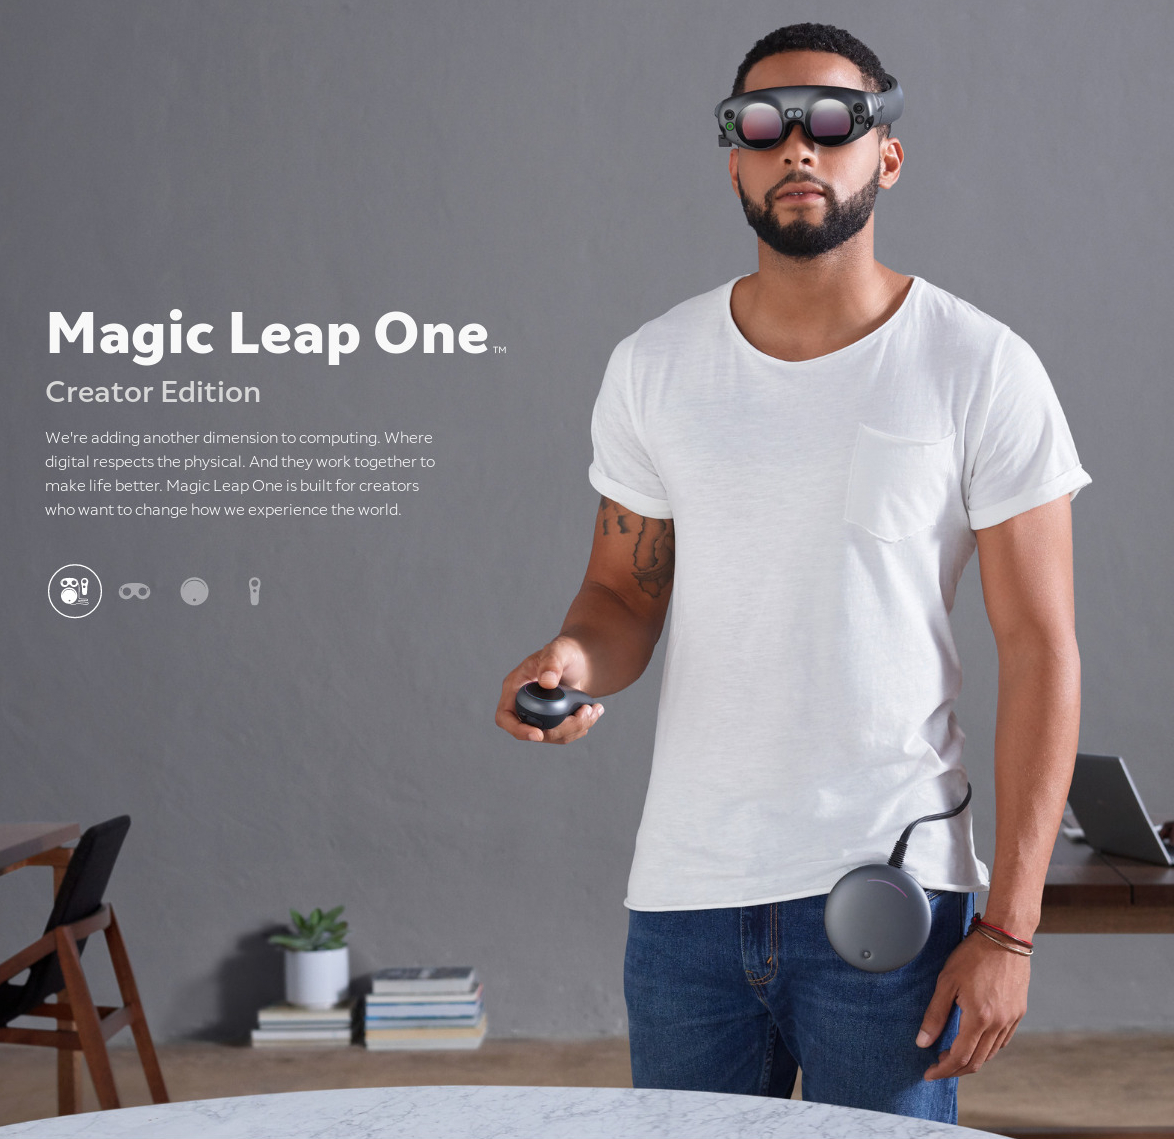
\includegraphics[width=0.45\textwidth]{figures/magic_leap.jpg}
	\caption{%
		Nutzer trägt die Magic Leap, bestehend aus drei Komponenten: \emph{Lightwear} (Brille), \emph{Lightpack} (Recheneinheit) und \emph{Control} (Controller).
		Quelle: \autocite{MagicLeap2018}
	}
	\label{fig:magic_leap}
\end{figure}

Ein weiteres Problem mit den bisherigen Ansätzen ist die Passivität der Navigationshinweise.
In der Regel reagieren die virtuellen Objekte nur in sofern auf die Nutzer, als dass sie ihre Positionen und Rotationen anpassen wenn die Nutzer sich bewegen.
Andere Interaktionen (zum Beispiel das \enquote{Berühren} von virtuellen Objekten) werden häufig nicht implementiert.
Dies führt dazu, dass tatsächlich nur der Navigationsvorgang selbst augmentiert wird.
Anwendungen wie zum Beispiel das Planen von Routen oder das direkte Interagieren mit der Karte sind nicht möglich.

Ein anderer Bereich, in dem Navigation eine große Rolle spielt, sind digitale Spiele.
Insbesondere stellt Navigation in \emph{Open-World}-Spielen (OWS) eine Herausforderung dar.
OWS sind Spiele, in denen sich Spieler frei in einer vergleichsweise großen Spielwelt bewegen können (im Kontrast zu Spielen mit stark eingegrenzten \enquote{Leveln} wie z.B. \emph{Super Mario} oder Rennspielen).
Diese Bewegungsfreiheit geht mit einer gewissen Anforderung an die Navigationsfähigkeiten der Spieler einher.
Um die Spieler zu unterstützen verwenden solche Spiele diverse Navigationshinweise.
\textcite{Lodts2015} gibt einen Überblick über verwendete Hinweise in OWS.

\begin{figure}
	\centering
	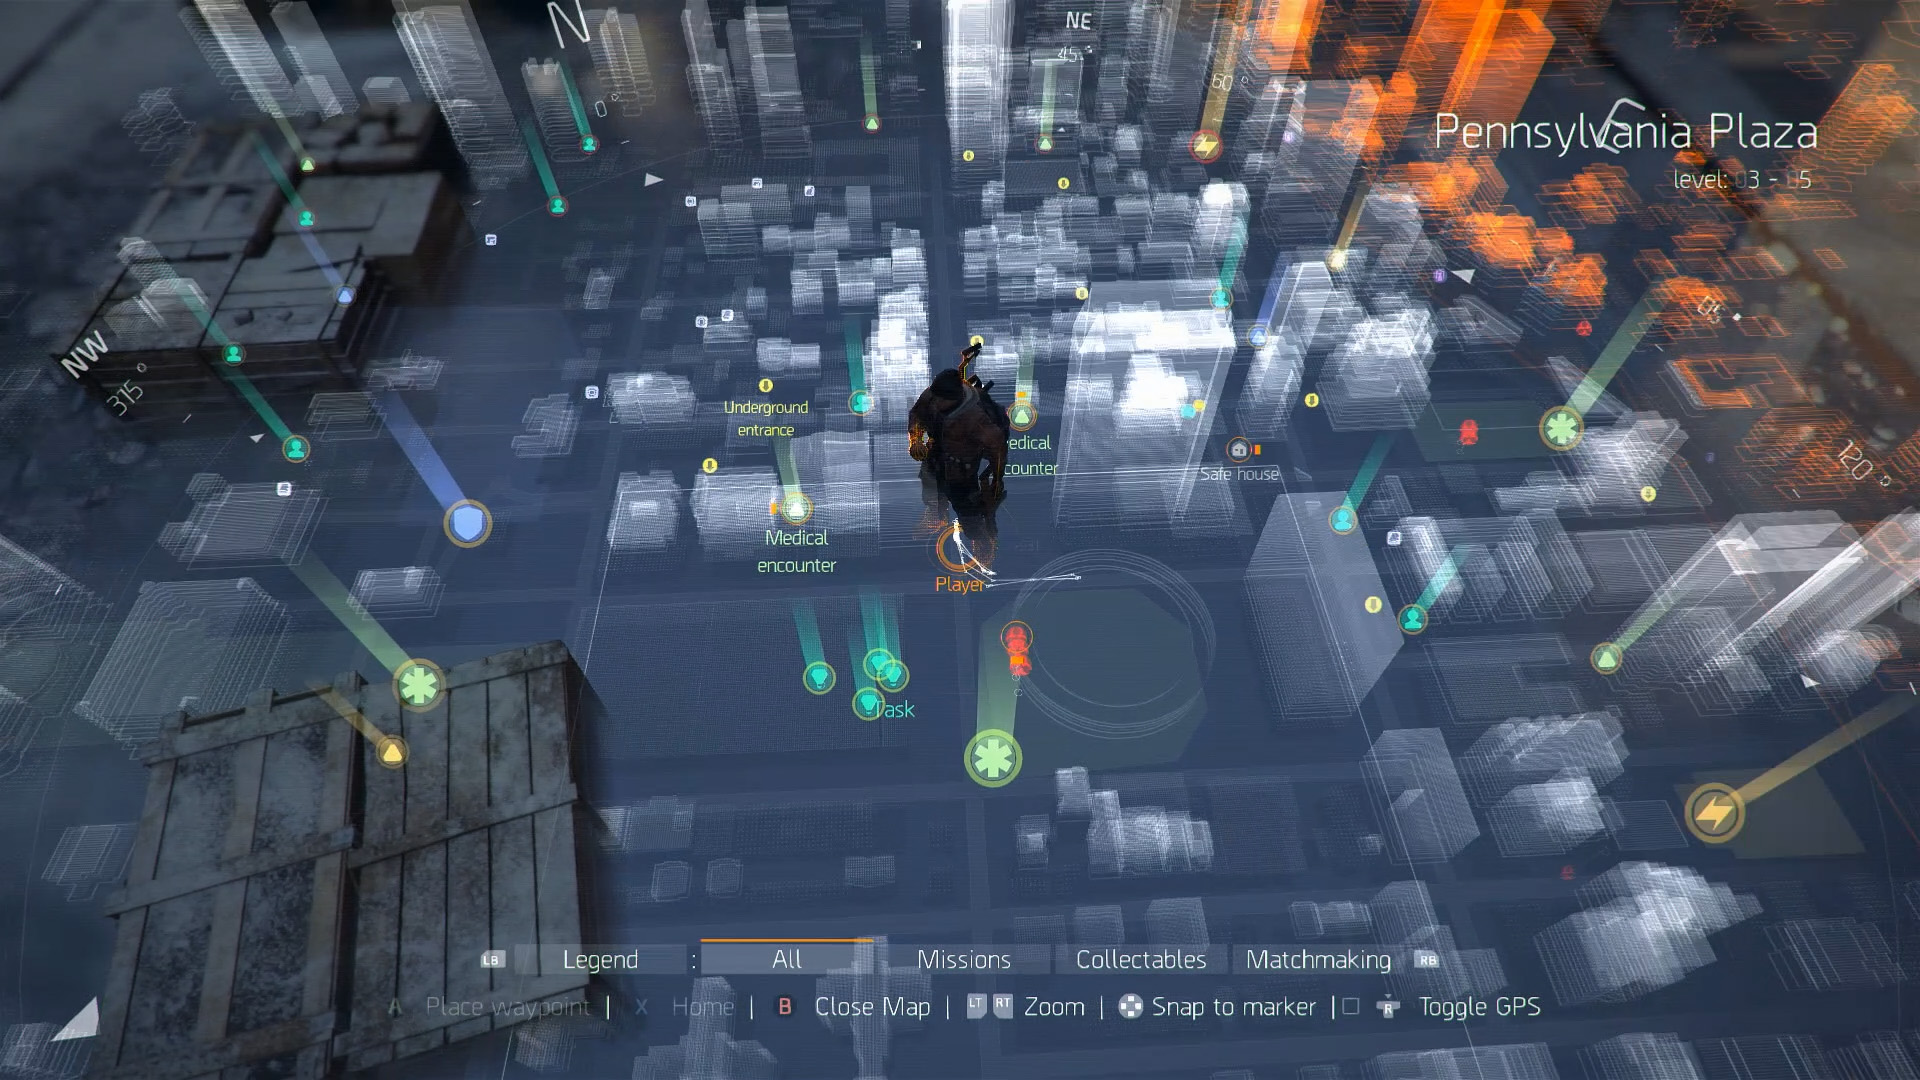
\includegraphics[width=0.8\textwidth]{figures/the_division_megamap.jpg}
	\caption{%
		Die Karte in Tom Clancy's: The Division wird in der Umgebung des Charakters angezeigt.
		Die Skalierung kann verändert werden, wodurch sich die Details der gezeigten Gebäude anpassen.
		Quelle: \autocite{MYDIVISION.NET2014}
	}
	\label{fig:the_division_megamap}
\end{figure}

Von besonderem Interesse ist die sogenannte \emph{\enquote{Mega-Map}} aus \emph{Tom Clancy's: The Division} \autocite{Ubisoft2018}.
Im Gegensatz zu den meisten anderen Navigationshinweisen handelt es sich hier nicht um ein passives System.
Es wird eine interaktive, dreidimensionale (3D) Karte im unmittelbaren Umfeld des Spielers dargestellt.
\autoref{fig:the_division_megamap} zeigt, wie die Karte im Spiel aussieht.
Die Karte wird so platziert, dass Spieler in der Kartenansicht an der Stelle stehen, die deren Position in der Spielwelt entspricht.
Damit ist die Karte immer mit dem jeweiligen Standort registriert.
Das Besondere ist, dass diese Karte Spielern aktiv Interaktionen anbietet:
die Spieler können zum Beispiel Gebäude auswählen, um mehr Informationen zu erhalten oder Wegpunkte zu setzen.
Sie geht über die Funktionen eines regulären Navigations\emph{hinweises} hinaus.
% TODO: Hmm kling doof...
Die Karte dient als Interface für Entdeckung und Exploration und kann somit andere Navigationshelfer kontrollieren und beeinflussen.

Basierend auf dem Konzept der Mega-Map ergibt sich die grundlegende Fragestellung dieser Masterarbeit:
\begin{quote}
	\itshape
	Können die Navigationsmetaphern aus Open-World-Spielen in die \enquote{reale} Welt mittels Augmented Reality übertragen werden, um so die Navigationssituation für Nutzer zu verbessern?
\end{quote}

Um diese Frage zu beantworten soll eine Mega-Map-Anwendung nach dem Vorbild aus Tom Clancy's: The Division für ein MR-HMD entwickelt werden.
Dabei soll die Karte in Echtzeit navigierbar sein.
Weiterhin soll die Karte dynamisch sein.
Das heißt, dass kein vorbereitetes 3D-Modell für die Umgebung verwendet wird.
Stattdessen soll die Karte durch Umgebungsinformationen, den Tiefensensoren des HMDs sowie der \emph{Google Maps} Programmierschnittstelle (\emph{Application Programming Interface} / API) dynamisch generiert werden.
Außerdem soll die Anwendung zwei Modi unterstützen: Einerseits soll die Karte z.B. durch Gesten und/oder Sprachkommandos interaktiv sein.
So könnten Routen geplant oder Informationen abgerufen werden.
Sobald eine Route festgelegt ist sollen entsprechende Navigationshinweise auf dem Weg zum Ziel angezeigt werden.

Einige der Fragen und Probleme, die in dieser Arbeit beantwortet bzw. behandelt werden sollen, sind:
\begin{description}
\item[Verankerung der Karte in Realität]
	Die Karte soll nicht einfach nur der realen Umgebung überlagert werden.
	Tatsächlich soll die geometrische Struktur der Umgebung für die Karte und die Navigationshinweise genutzt werden.
	Z.B. könnten Pfeile und Textinformationen an Gebäudefassaden angezeigt werden.
	Reale Oberflächen können wiederum als haptische Eingabeflächen dienen.
\item[Übertragbarkeit \emph{Third-Person} nach \emph{First-Person}]
	Das Verwenden eines HMDs kommt einem Spiel in der First-Person-Perspektive gleich.
	Viele OWS (wie auch The Division) verwenden jedoch eine Third-Person-Perspektive.
	Daher muss ermittelt werden, inwiefern sich das Konzept der Mega-Map sowie der verschiedenen Navigationshinweise auf die \enquote{Ego-Perspektive} übertragen lässt.
\item[Wie ist das passive Verhalten der Mega-Map?]
	Bei der Entwicklung der Anwendung muss darauf geachtet werden, wie sich die Karte hält wenn sich die Nutzer bewegen.
	Was passiert z.B., wenn Nutzer vorwärts laufen oder sich drehen während die Karte angezeigt wird?
\item[Wie ist das aktive Verhalten der Mega-Map?]
	Da mit der Karte interagiert werden soll müssen sinnvolle und nutzerfreundliche Interaktionsmöglichkeiten implementiert werden.
\item[Integration in Umgebung]
	Einerseits soll die Karte so dargestellt werden, dass die Überlappung mit der Umgebung korrekt dargestellt wird (Stichwort \emph{Occlusion}).
	Andererseits muss auch ermittelt werden, wie die Karte einer größeren Umgebung sinnvoll auf einem kleinen Bereich angezeigt werden kann.
	Außerdem wäre hier auch zu beachten, ob es einen Unterschied zwischen Indoor- und Outdoor-Anwendungen gibt.
\end{description}

Die Effektivität der entwickelten Anwendung zugunsten der Navigationssituation sowie ihre Nutzbarkeit sollte schließlich durch eine Evaluation nachgewiesen werden.

\vspace{1em}
\hrule
\printbibliography[nottype=online]
\printbibliography[title={Online Referenzen}, type=online]

\end{document}
